\documentclass{article}
\setlength{\oddsidemargin}{0.25 in}
\setlength{\evensidemargin}{-0.25 in}
\setlength{\topmargin}{-0.6 in}
\setlength{\textwidth}{6.5 in}
\setlength{\textheight}{8.5 in}
\setlength{\headsep}{0.75 in}
\setlength{\parindent}{0 in}
\setlength{\parskip}{0.1 in}

\usepackage{amsmath,amsfonts,graphicx}
\usepackage{hyperref}
\usepackage{enumitem}

\newcounter{lecnum}
\renewcommand{\thepage}{\thelecnum-\arabic{page}}
\renewcommand{\thesection}{\thelecnum.\arabic{section}}
\renewcommand{\theequation}{\thelecnum.\arabic{equation}}
\renewcommand{\thefigure}{\thelecnum.\arabic{figure}}
\renewcommand{\thetable}{\thelecnum.\arabic{table}}

%
% The following macro is used to generate the header.
%
\newcommand{\lecture}[4]{
   \pagestyle{myheadings}
   \thispagestyle{plain}
   \newpage
   \setcounter{lecnum}{#1}
   \setcounter{page}{1}
   \noindent
   \begin{center}
   \framebox{
      \vbox{\vspace{2mm}
    \hbox to 6.28in { {\bf CS 768: Learning With Graphs
        \hfill Autumn 2020-2021} }
       \vspace{4mm}
       \hbox to 6.28in { {\Large \hfill Lecture #1: #2  \hfill} }
       \vspace{2mm}
       \hbox to 6.28in { {\it Instructor: Prof. Abir De \hfill Scribe: #4} }
      \vspace{2mm}}
   }
   \end{center}
   \markboth{Lecture #1: #2}{Lecture #1: #2}
}

%Use this command for a figure; it puts a figure in wherever you want it.
%usage: \fig{NUMBER}{SPACE-IN-INCHES}{CAPTION}
\newcommand{\fig}[3]{
            \vspace{#2}
            \begin{center}
            Figure \thelecnum.#1:~#3
            \end{center}
    }
% Use these for theorems, lemmas, proofs, etc.
\newtheorem{theorem}{Theorem}[lecnum]
\newtheorem{lemma}[theorem]{Lemma}
\newtheorem{proposition}[theorem]{Proposition}
\newtheorem{claim}[theorem]{Claim}
\newtheorem{corollary}[theorem]{Corollary}
\newtheorem{definition}[theorem]{Definition}
\newenvironment{proof}{{\bf Proof:}}{\hfill\rule{2mm}{2mm}}

% **** IF YOU WANT TO DEFINE ADDITIONAL MACROS FOR YOURSELF, PUT THEM HERE:
\newcommand{\Sim}{\text{sim}}

\begin{document}

\lecture{3}{Examples of Aggregate and Per-Node Sampling}{}{Shubham Sharma and Jennish Dharma J J}

In the last lecture, we had an overview of Aggregated Sampling and Per-Node sampling. In this lecture, we'll see some applications and examples of both these sampling. In section \ref{sec1}, we'll again visit the necessity for train test split. In section \ref{sec2}, we'll see the methods and need to split into train and test set. In section \ref{sec3}, we'll see the application of both Aggregate and Per-Node Sampling. Section \ref{sec4} contains some examples of both Aggregate and Per-Node Sampling.

\section{Necessity for Train Test split}\label{sec1}
\qquad In Link Prediction, our task is to rank the non-edges as the graph evolves. In most cases, we only get a snapshot a graph and we can't wait for the graph to evolve to see which turns out to be edges to evaluate the model we had trained. Therefore, we have to evaluate the Link Predictor using the current snapshot of the graph itself and to do this, we split the graph into test and train edges and non edges. 

\section{Train and Test Split}\label{sec2}
\qquad To obtain a train and a test set from a given graph, we choose a fraction of edges from the graph to make a train set and remaining edges to form a test set. Similarly, we do the same for non edges. Non edges are also split into train and test so that we don't use any information about the non edges that we are going to evaluate against later. Therefore, while training a link predictor using the training set, we have to make sure that we use only the labels of the non edges other than the ones in test set and not use any information of the no edges in test set. It is not possible to not use information form the test set. For example, when we construct features for each node $f_{u}$ to train the LP, we have to know the relationship between 2 nodes and thus we have to incorporate the fact that it is not an edge and thus information leaks from test set. But since the fraction of non edges in test set is much smaller than that is training set we can neglect the effects caused by this in features $f_{u}$.  

\section{Application}\label{sec3}
\begin{enumerate}
    \item Applications of Aggregrate Sampling
    \begin{itemize}
        \item Predicting which two authors are going to collaborate in a particular topic from citation graphs.
        \item Predicting which k connections are potentially lethal in a social network.
        \item Understanding reaction mechanisms.
        \item Predicting interactions in Protein Protein Interaction (PPO) network
    \end{itemize}
    
    \item Applications of node specific sampling
    \begin{itemize}
        \item Used when we want to do well across all nodes
        \item Recommending k users to an user to send friend requests in Facebook
        \item Recommending m movies to an user in Netflix
    \end{itemize}
\end{enumerate}

\section{Examples}\label{sec4}
Let G be the graph with V=$\{$W,V,X,Y,U,Z$\}$ and E=$\{$WV,VX,XY,YU,UZ,ZW,UV$\}$ are the given edges as shows in the figure \ref{fig:Graph}. All other links are the non-edges that are denoted by the dotted lines. In the link prediction task, ideally, we want to rank the non-edges. So, there are different likelihoods across these dotted lines and we want to rank them. Let us now try to split the graph into train and test set.(Note that we are splitting as $50\%$Train + $50\%$Test, so we can consider the splits in the below subsections as either train or test)
\begin{figure}[h!]
    \centering
    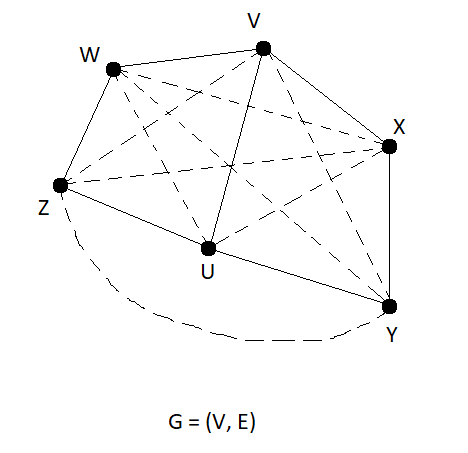
\includegraphics[width=0.3\linewidth]{graph.png}
    \caption{Graph}
    \label{fig:Graph}
\end{figure}

\subsection{Aggregate Sampling($50\%$Train + $50\%$Test)}
\begin{enumerate}
    \item We spilt both edges and non-edges into $50\%$Train + $50\%$Test.
    \item Here the Graph \ref{fig:Aggregate_Sampling} is the train set with lines as edges and dotted lines as non edges. All other connections are what we want to predict with our LP Algorithm. 
    \item However, in case of features extraction of a particular node, there would be problem with the nodes like X, so, one way is  we can assume that test non-edges are the training non edges, but test edges are training non edges.
\end{enumerate}
\begin{figure}[h!]
    \centering
    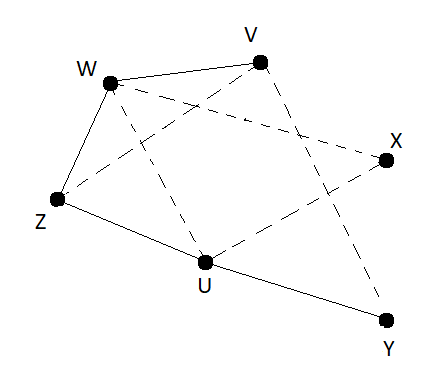
\includegraphics[width=0.3\linewidth]{aggregate.png}
    \caption{Aggregate Sampling}
    \label{fig:Aggregate_Sampling}
\end{figure}


\subsection{Per-Node Sampling($50\%$Train + $50\%$Test)}
\begin{enumerate}
    \item We spilt both edges and non-edges into $50\%$Train + $50\%$Test for each node in this case.
    \item Graph \ref{fig:Aggregate_Sampling} shows how we can split edges and non-edges for each node. It contains the split for nodes X,U,V. We can find the split for other nodes similarly.
    \item In cases like let say Y has selected U as a node with edge while training, but U has not selected Y as a node with edge while training, then we can choose randomly whether or not that edge UY should be in training set or not.
\end{enumerate}
\begin{figure}[h!]
    \centering
    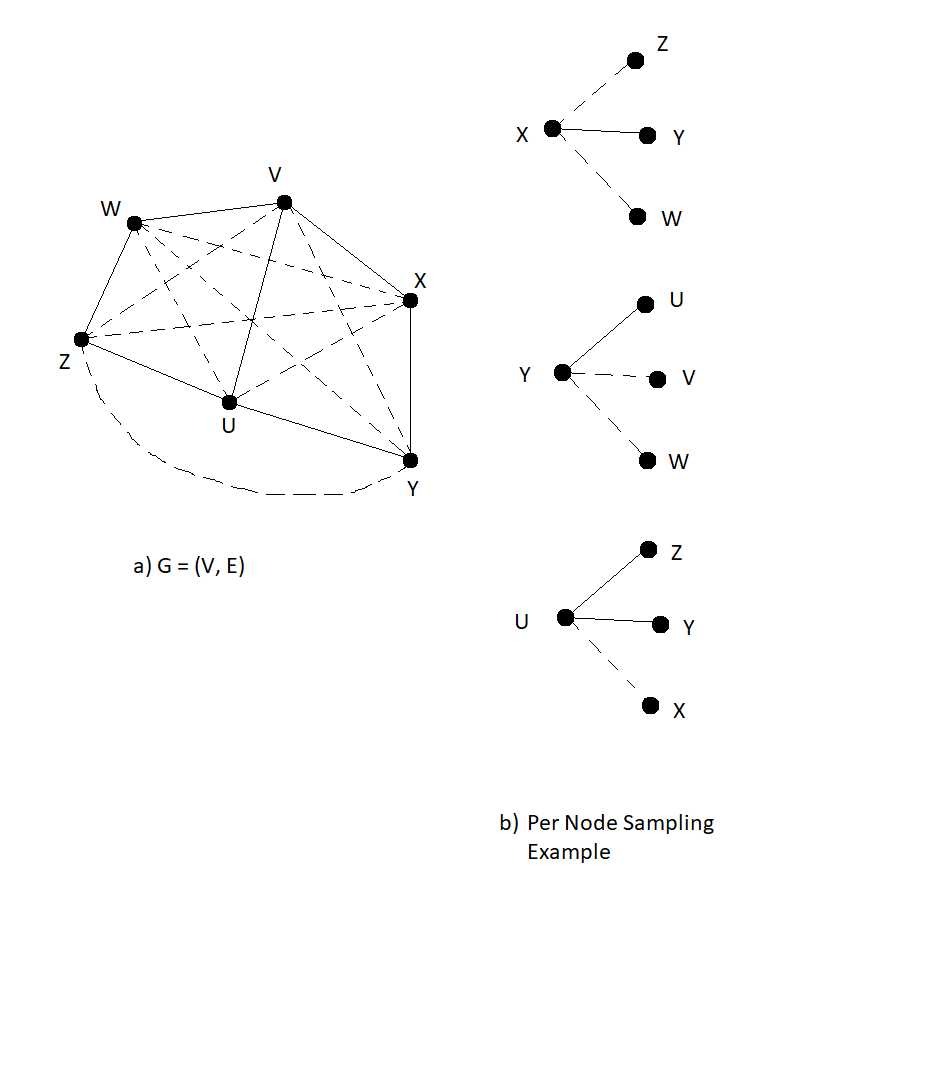
\includegraphics[width=0.7\linewidth]{per_node.png}
    \caption{Per Node Sampling}
    \label{fig:per_node}
\end{figure}

\end{document}
